\documentclass[11pt, addpoints, answers]{exam}

\usepackage{amsmath, amssymb, euler}
\usepackage{amsthm}
\usepackage{xcolor}
\usepackage{proof}
\usepackage{algorithm, algorithmicx, algpseudocode}
\usepackage{tikz, tikz-qtree, drawstack}
\usepackage[shortlabels]{enumitem}

\usetikzlibrary{graphs}
\tikzset{every tree node/.style={minimum width=2em,draw,circle},
	blank/.style={draw=none},
	edge from parent/.style=
	{draw,edge from parent path={(\tikzparentnode) -- (\tikzchildnode)}},
	level distance=1.2cm}

% For inserting code snippets.
\usepackage{listings}
\lstset{
    columns = fixed,
    basewidth = {0.5em},
    breaklines = true,
    backgroundcolor = \color{white},
    keywordstyle = \color[RGB]{40, 40, 255},
    numberstyle = \footnotesize\color{darkgray},
    commentstyle = \ttfamily\color{violet},
    basicstyle = \ttfamily,
    stringstyle = \ttfamily\color[RGB]{128, 0, 0},
    showstringspaces = false,
    language = {[11]C++},
    escapechar = \@
}
\lstnewenvironment{cpp}[1][]{\lstset{language = {[11]C++}, #1}}{}

\usepackage{tikz}

% headers, footers, titles
\newcommand{\CourseName}{CS101 Algorithms and Data Structures}
\newcommand{\HomeworkNO}{Homework 4}
\newcommand{\DueDate}{Due date: 23:59, November 5th, 2023}

\pagestyle{headandfoot}
\runningheadrule
\runningheader{\CourseName}{\HomeworkNO}{\DueDate}
\runningfooter{}{\thepage}{}

\title{
	\CourseName\\
	Fall 2023\\
	\HomeworkNO
}
\author{}
\date{\DueDate}

% formats of questions, choices, points, etc.
\qformat{\bf\thequestion. (\totalpoints\ points) \thequestiontitle\hfill}
\pointname{'}
\CorrectChoiceEmphasis{\bf\color{blue}}
\SolutionEmphasis{\color{blue}}

% We frequently use this font.
\newcommand{\ttt}{\texttt}

\begin{document}

\maketitle

\begin{enumerate}
	\item Please write your solutions in English.
	\item Submit your solutions to gradescope.com.
	\item Set your FULL name to your Chinese name and your STUDENT ID correctly in Account Settings.
	\item If you want to submit a handwritten version, scan it clearly. \ttt{CamScanner} is recommended.
	\item When submitting, match your solutions to the problems correctly.
	\item No late submission will be accepted.
	\item Violations to any of the above may result in zero points.
\end{enumerate}

\newpage

{\large\textbf{Notes}:}

\begin{enumerate}
	\item Some problems in this homework requires you to design divide-and-conquer algorithm. When grading these problems, we will put more emphasis on how you reduce a problem to a smaller size problem and how to combine their solutions with divide-and-conquer strategy. 
	\item Your answer for these problems {\color{red}\textbf{should}} include:
	\begin{enumerate}
		\item {\color{red} \textbf{Clear description} of your algorithm design in \textbf{natural language}, with \textbf{pseudocode} if necessary.}
		\item {\color{red}Run-time Complexity Analysis}
            \item {Proof of Correctness (If required)}
	\end{enumerate}
    \item Your answer for these problems is {\color{red}not allowed to include real C or C++ code}.
	\item In your description of algorithm design, you should describe each step of your algorithm clearly.
	\item You are encouraged to write pseudocode to facilitate explaining your algorithm desgin, though this is not mandatory. If you choose to write pseudocode, please give some additional descriptions to make your pseudocode intelligible.
	\item You are recommended to finish the algorithm design part of this homework with \LaTeX.
\end{enumerate}

\begin{questions}

\titledquestion{(DP Example) Maximum Subarray Problem}

Given an array $A=\langle A_1, \dots, A_n\rangle$ of $n$ elements, please design a dynamic programming algorithm to find a contiguous subarray whose sum is maximum.

\vspace{0.05in}
{\large\textbf{Notes:}} \textcolor{red}{(MUST READ!)}

\begin{enumerate}
    \item Problems in this homework require you to design \textbf{dynamic programming} algorithms. When grading these problems, we will put more emphasis on how you define your subproblems, whether your Bellman equation is correct and correctness of your complexity analysis.
    \item \textbf{Define your subproblems clearly.} Your definition should include the variables you choose for each subproblem and a brief description of your subproblem in terms of the chosen variables.
    \item Your \textbf{Bellman equation} should be a recurrence relation whose \textbf{base case} is well-defined. You can breifly \textbf{explain each term in the equation} if necessary, which might improve the readability of your solution and help TAs grade it. 
    \item Analyse the \textbf{runtime complexity} of your algorithm in terms of $\Theta(\cdot)$ notation.
    \item You only need to calculate the optimal value in each problem of this homework and you don't have to back-track to find the optimal solution.
\end{enumerate}

% utilities you might need for wrting Bellman equations
\newcommand{\maxi}[2]{\max\left\{\substack{#1\\#2}\right\}}	% usage: \maxi{a}{b}
\newcommand{\mini}[2]{\min\left\{\substack{#1\\#2}\right\}}	% usage: \mini{a}{b}
\newcommand{\case}[1]{\text{if}\ #1}	% usage: \case{$i > 1$}
\newcommand{\otherwise}{\text{otherwise}}	% usage: \otherwise

\vspace{0.05in}
\begin{parts}
\part[0] Define the subproblems: $OPT(i)=$ the maximum sum of subarrays of $A$ ending with $A_i$. Give your Bellman equation to solve the subproblems.
\begin{solution}
    \[
        OPT(i)=
        \begin{cases}
            A_1                       & \case{i=1} \\
            \max \{A_i,A_i+OPT(i-1)\} & \otherwise
        \end{cases}
    \]
    \paragraph{Explanation:} (NOT Required)
    \begin{itemize}
        \item The $1$st term in $\max$: only take $A_i$
        \item The $2$nd term in $\max$: take $A_i$ together with the best subarray ending with $A_{i-1}$
    \end{itemize}
\end{solution}

\part[0] What is the answer to this question in terms of $OPT$?
\begin{solution}
    \[ \max_{i\in\{1, 2, \dots, n\}} OPT(i) \]
\end{solution}

\part[0] What is the runtime complexity of your algorithm? (answer in $\Theta(\cdot)$)
\begin{solution}
    $\Theta(n)$
\end{solution}
\end{parts}


\newpage

\titledquestion{Multiple Choices}

Each question has \textbf{one or more} correct answer(s). Select all the correct answer(s). For each question, you will get 0 points if you select one or more wrong answers, but you will get 1 point if you select a non-empty subset of the correct answers.

Write your answers in the following table.

\begin{table}[htbp]
    \centering
    \begin{tabular}{|p{2cm}|p{2cm}|p{2cm}|p{2cm}|}
        \hline
        (a) & (b) & (c) \\
        \hline
        %%%%%%%%%%%%%%%%%%%%%%%%%%%%%%%%%%%%%%%%%%%%%%%%%%%%%%%%%%
        % YOUR ANSWER HERE.
            &     &     \\
        %%%%%%%%%%%%%%%%%%%%%%%%%%%%%%%%%%%%%%%%%%%%%%%%%%%%%%%%%%
        \hline
    \end{tabular}
\end{table}

\begin{parts}
        
    \part[3] Which of the following sorting algorithms can be implemented as the stable ones?
    \begin{choices}
        \choice  Insertion-Sort 
        \choice Merge-Sort
        \choice Quick-Sort (always picking the first element as pivot)
        \choice None of the above
    \end{choices}
    
    \part[3] Which of the following implementations of quick-sort take \(\Theta(n\log n)\) time in the \textbf{worst case}?
    
    \begin{choices}
        \choice Randomized quick-sort, i.e. choose an element from \(\left\{a_l,\cdots,a_r\right\}\) randomly as the pivot when partitioning the subarray \(\langle a_l,\cdots,a_r\rangle\).
        \choice When partitioning the subarray \(\langle a_l,\cdots,a_r\rangle\) (assuming \(r-l\geqslant 2\)), choose the median of \(\left\{a_x,a_y,a_z\right\}\) as the pivot, where \(x,y,z\) are three different indices chosen randomly from \(\{l,l+1,\cdots,r\}\).
        \choice When partitioning the subarray \(\langle a_l,\cdots,a_r\rangle\) (assuming \(r-l\geqslant 2\)), we first calculate \(q = \frac{1}{2} (a_{\max} + a_{\min})\) where \(a_{\max}\) and \(a_{\min}\) are the maximum and minimum values in the current subarray respectively. Then we traverse the whole subarray to find \(a_m \; s.t. \left|a_m - q\right| = \min_{i=l}^r \left|a_i - q\right|\) and choose \(a_m\) as the pivot.
        \choice None of the above.
    \end{choices}

    \part[3] Which of the following statements are true?
    
    \begin{choices}
        \choice If \(T(n) = 2T(\frac{n}{2}) + O(\sqrt{n})\) with \(T(0) = 0\) and \(T(1) = 1\), then \(T(n) = \Theta(n)\).
        \choice If \(T(n) = 4T(\frac{n}{2}) + O(n^2)\) with \(T(0) = 0\) and \(T(1) = 1\), then \(T(n) = \Theta(n^2 \log n)\).
        \choice If \(T(n) = 3T(\frac{n}{2}) + \Theta(n^2)\) with \(T(0) = 0\) and \(T(1) = 1\), then \(T(n) = \Theta(n^2)\).
        \choice If the run-time $T(n)$ of a divide-and-conquer algorithm satisfies \(T(n) = aT(\frac{n}{b}) + f(n)\) with \(T(0) = 0\) and \(T(1) = 1\), we may deduce that the run-time for merging solutions of $a$ subproblems of size $\frac{n}{b}$ into the overall one is $f(n)$.      
    \end{choices}

\end{parts}

\newpage

\titledquestion{Element(s) Selection}

\begin{parts}
  \part{} \textbf{Selection of the \(k\)-th Minimal Value} \par
  In this part, we will design an algorithm to find the \(k\)-th minimal value of a given array \(\langle a_1,\cdots,a_n\rangle\) of length \(n\) with \emph{distinct} elements for an integer \(k\in[1,n]\). We say \(a_x\) is the \(k\)-th minimal value of \(a\) if there are exactly \(k-1\) elements in \(a\) that are less than \(a_x\), i.e.
  \[\left|\left\{i\mid a_i<a_x\right\}\right|=k-1.\]
  Consider making use of the `\textbf{partition}' procedure in quick-sort. The function has the signature
  \begin{cpp}
    int partition(int a[], int l, int r);
  \end{cpp}
  which processes the subarray \(\langle a_l,\cdots,a_r\rangle\). It will choose a pivot from the subarray, place all the elements that are less than the pivot before it, and place all the elements that are greater than the pivot after it. After that, the index of the pivot is returned.

  Our algorithm to find the \(k\)-th minimal value is implemented below.
  \begin{cpp}
    // returns the k-th minimal value in the subarray a[l],...,a[r].
    int kth_min(int a[], int l, int r, int k) {
        auto pos = partition(a, l, r), num = pos - l + 1;
        if (num == k)
        return a[pos];
        else if (num > k)
        return kth_min(l, pos - 1, k);
        else
        return kth_min(pos + 1, r, k - num);
      }
  \end{cpp}
  By calling \lstinline{kth_min(a, 1, n, k)}, we will get the answer.

  \begin{subparts}
    \subpart[2] Fill in the blanks in the code snippet above.
    \subpart[2] What's the time complexity of our algorithm in the \textbf{worst case}? Please answer in the form of \(\Theta(\cdot)\) and fully justify your answer.
    \begin{solution}
      %%%%%%%%%%%%%%%%%%%%%%%%%%%%%%%%%%%%%%%%%%%%%%%%%
      % Replace `\vspace{2.5in}' with your answer.
      $\Theta(n^2)$
      \begin{proof}
        The worst case is when the pivot is always the largest or smallest pivotable element in the array. In this case, $T(n) = T(n-2) + \theta(n)$.
        so the worst case is $\Theta(n^2)$.
      \end{proof}
      %%%%%%%%%%%%%%%%%%%%%%%%%%%%%%%%%%%%%%%%%%%%%%%%%
    \end{solution}
  \end{subparts}

  \newpage

  \part{} \textbf{Batched Selection} \par

  Despite the worse-case time complexity of the algorithm in part(a), it actually finds the $k$-th minimal value of \(\langle a_1,\cdots,a_n\rangle\) in expected $O(n)$ time. In this part, we will design a divide-and-conquer algorithm to answer $m$ selection queries for distinct $k_1, k_2, \cdots, k_m$ where $k_1 < k_2 < \cdots < k_m$ on an given array $a$ of n distinct integers (i.e. finding the $k_1$-th, $k_2$-th,$\cdots$,$k_m$-th minimal elements of $a$) and here $m$ satisfies $m = \Theta(\log n)$.

  \begin{subparts}
    \subpart[1] Given that $x$ is the $k_p$-th minimal value of $a$ and $y$ is the $k_q$-th minimal value of $a$ for $1 \leq p < q \leq m$, which of the following is true?

    \begin{oneparcheckboxes}
      \CorrectChoice $x < y$
      \choice $x = y$
      \choice $x > y$
    \end{oneparcheckboxes}



    \subpart[2] Suppose by calling the algorithm in part(a), we have already found $z$ to be the $k_l$-th minimal value of $a$ for $1 < l < m$. Let $L = \left\{a_i \mid a_i < z\right\}$ and $R = \left\{a_i \mid a_i > z\right\}$. What can you claim about the $k_1$-th,$\cdots$,$k_{l-1}$-th minimal elements of $a$ and the $k_{l+1}$-th,$\cdots$,$k_{m}$-th minimal elements of $a$?

    \begin{solution}
      %%%%%%%%%%%%%%%%%%%%%%%%%%%%%%%%%%%%%%%%%%%%%%%%%
      % Replace `\vspace{1in}' with your answer.
      $k_1$-th,$\cdots$,$k_{l-1}$-th minimal elements are in $L$ and the $k_{l+1}$-th,$\cdots$,$k_{m}$-th minimal elements are in $R$.
      %%%%%%%%%%%%%%%%%%%%%%%%%%%%%%%%%%%%%%%%%%%%%%%%%    
    \end{solution}

    \subpart[6] Based on your answers of previous parts, design a divide-and-conquer algorithm, \textbf{which calls the algorithm in part(a) as a subroutine}, for this problem. Your algorithm should runs in \textbf{expected} $O(n \log m) = O(n \log \log n)$ time. Any algorithms that run in $\Omega(n \log n)$ time will get no credit. Make sure to provide \textbf{clear description} of your algorithm design in \textbf{natural language}, with \textbf{pseudocode} if necessary.

    \begin{solution}
      %%%%%%%%%%%%%%%%%%%%%%%%%%%%%%%%%%%%%%%%%%%%%%%%%
      % Replace `\vspace{2.5in}' with your answer.
      $ $\\
      Assuming $k_1$,$\cdots$,$k_{m}$ are passed in as an array $k$.
      \begin{enumerate}
        \item
              Allocate an array $b$ with length $m$.
        \item
              Choose the median of $k_1$,$\cdots$,$k_{m}$: $k_j$.
        \item
              Calls the algorithm in (a) to find the element of $k_j$ minimal elements of $a$.
        \item
              Get the index of the element $k_j$ minimal element of $a$.
        \item
              Store the element in $b[j]$.
        \item
              If $k$'s length is 1, return $b$.
        \item
              Partition the array into two parts: $L$ and $R$ using the $k_j$ minimal elements as pivot.
        \item
              Recursively call the algorithm on $L$ to find the $k_1$-th,$\cdots$,$k_{l-1}$-th minimal elements.
        \item
              Store the returned elements in $b$.
        \item
              Recursively call the algorithm on $R$ to find the $k_{l+1}$-th,$\cdots$,$k_{m}$-th minimal elements.
        \item
              Store the returned elements in $b$.
        \item
              Return $b$.
      \end{enumerate}
      %%%%%%%%%%%%%%%%%%%%%%%%%%%%%%%%%%%%%%%%%%%%%%%%%    
    \end{solution}

    \subpart[2] Provide your reasoning for why your algorithm in the previous part runs in expected $O(n\log m)$ time using the \textbf{recursion-tree} method.
    \begin{solution}
      %%%%%%%%%%%%%%%%%%%%%%%%%%%%%%%%%%%%%%%%%%%%%%%%%
      % Replace `\vspace{3in}' with your answer.
      $ $\\
      The algorithm's time complexity is $T(m) = 2T(m/2) + O(n)$.
      The recursion tree of the algorithm is a binary tree with $\log m$ layers. So the total time is $O(n\log m)$.
      %%%%%%%%%%%%%%%%%%%%%%%%%%%%%%%%%%%%%%%%%%%%%%%%%      
    \end{solution}

  \end{subparts}

\end{parts}

\newpage

\titledquestion{Maximum area rectangle in histogram}

We are given a histogram consisting of $n$ parallel bars side by side, each of width $1$, as well as a sequence $A$ containing the heights of the bars where the height of the $i$th bar is $\mathbf{a}_i$ for $\forall \; i \in [n]$. For example, the figures below show the case where $n= 7$ and $A = \langle 6, 2, 5, 4, 4, 1, 3 \rangle$. Our goal is to find the maximum area of the rectangle placed inside the boundary of the given histogram with a \textbf{divide-and-conquer} algorithm. (Here you don't need to find which rectangle maximizes its area.)

Reminder: There do exist algorithms that solve this problem in linear time. However, you are \textbf{not allowed} to use them in this homework. Any other type of algorithms except the divide-and-conquer ones will get \textbf{no} credit.

\begin{figure}[htbp]
    \centering
    \begin{minipage}[t]{0.48\textwidth}
        \centering
        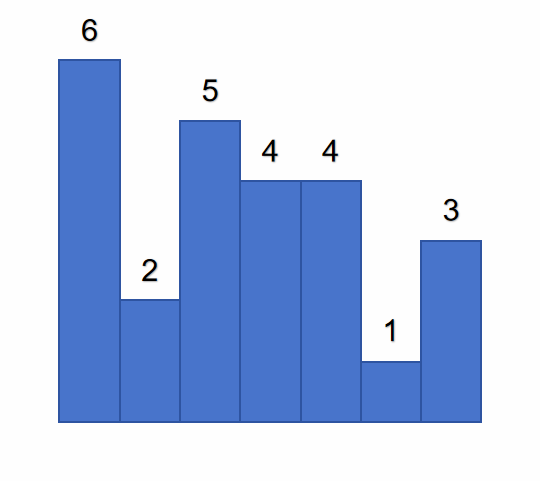
\includegraphics[width=6cm]{withnum.png}
        \caption{The Original Histogram}
    \end{minipage}
    \begin{minipage}[t]{0.48\textwidth}
        \centering
        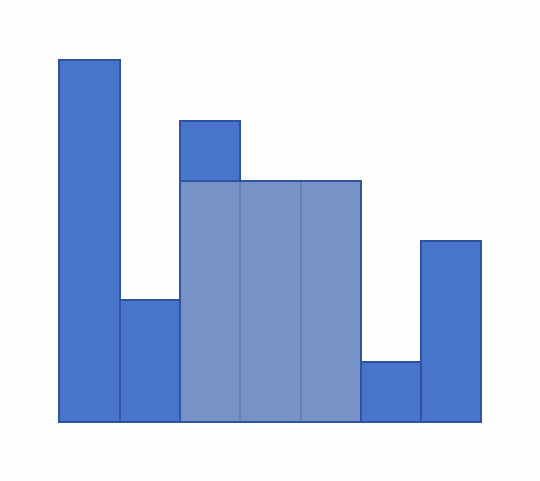
\includegraphics[width=6cm]{withrect.png}
        \caption{The Largest Rectangle in Histogram}
    \end{minipage}
\end{figure}

You may use $Rect(l, r, A)$ to represent the answer of the sub-problem w.r.t. the range $\left[l, r\right]$.

\begin{parts}
    \part[3] \textbf{Briefly} describe:
    \begin{enumerate}
        \item How would you divide the original problem into 2 sub-problems?
        \item Under what circumstances will the answer to the original problem not be covered by the answers of the 2 sub-problems?
        \item Given the answers of the 2 sub-problems, how would you get the answer of the original problem?
    \end{enumerate}
    
    \begin{solution}
    %%%%%%%%%%%%%%%%%%%%%%%%%%%%%%%%%%%%%%%%%%%%%%%%%
    % Replace `\vspace{2in}' with your answer.
    \vspace{2in}
    %%%%%%%%%%%%%%%%%%%%%%%%%%%%%%%%%%%%%%%%%%%%%%%%%
    \end{solution}

    \newpage
    
    \part[8] Based on your idea in part(a), design a \textbf{divide-and-conquer} algorithm for this problem. Make sure to provide \textbf{clear description} of your algorithm design in \textbf{natural language}, with \textbf{pseudocode} if necessary.
    
    \begin{solution}
    %%%%%%%%%%%%%%%%%%%%%%%%%%%%%%%%%%%%%%%%%%%%%%%%%
    % Replace `\vspace{7.5in}' with your answer.
    \vspace{7.5in}
    %%%%%%%%%%%%%%%%%%%%%%%%%%%%%%%%%%%%%%%%%%%%%%%%%
    \end{solution}

    \newpage
    
    \part[2] Provide the run-time complexity analysis of your algorithm in part (b). Make sure to include the \textbf{recurrence relation} of the run-time in your solution.
    
    \begin{solution}
    %%%%%%%%%%%%%%%%%%%%%%%%%%%%%%%%%%%%%%%%%%%%%%%%%
    % Replace `\vspace{3in}' with your answer.
    \vspace{3in}
    %%%%%%%%%%%%%%%%%%%%%%%%%%%%%%%%%%%%%%%%%%%%%%%%%
    \end{solution}
    
\end{parts}

\newpage

\titledquestion{Dividing with Creativity}

In this question, you are required analyze the run-time of algorithms with different dividing methods mentioned below. For each subpart except the third one, your answer should include:
\begin{enumerate}
    \item Describing the recurrence relation of the run-time $T(n)$. (Worth 1 point in 4)
    \item Finding the asymptotic order of the growth of $T(n)$ i.e. find a function $g$ such that $T(n) = O(g(n))$. Make sure your upper bound for $T(n)$ is tight enough. (Worth 1 point in 4)
    \item Show your \textbf{reasoning} for the upper bound of $T(n)$ or your process of obtaining the upper bound starting from the recurrence relation step by step. (Worth 2 points in 4)
\end{enumerate}

In each subpart, you may ignore any issue arising from whether a number is an integer as well as assuming \(T(0) = 0\) and \(T(1) = 1\). You can make use of the Master Theorem, Recursion Tree or other reasonable approaches to solve the following recurrence relations.

\begin{parts}
    \part[4] An algorithm $\mathcal{A}_1$ takes $\Theta(n)$ time to partition the original problem into 2 sub-problems, one of size $\lambda n$ and the other of size $(1-\lambda)n$ (here $\lambda \in \left(0, \frac{1}{2}\right)$), then recursively runs itself on both of the 2 sub-problems and finally takes $\Theta(n)$ time to merge the answers of the 2 sub-problems.

    \begin{solution}
        %%%%%%%%%%%%%%%%%%%%%%%%%%%%%%%%%%%%%%%%%%%%%%%%%
        % Replace `\vspace{5in}' with your answer.
        \begin{enumerate}
            \item
                  The recurrence relation for the algorithm can be expressed as:
                  $$T(n) = T(\lambda) + T((1-\lambda)) + O(n)$$

            \item
                  The overall time complexity is:
                  $$T(n) = O(n \log_{\frac{1}{-\lambda}}n)$$

            \item
        \end{enumerate}
        \vspace{3in}

        %%%%%%%%%%%%%%%%%%%%%%%%%%%%%%%%%%%%%%%%%%%%%%%%%    
    \end{solution}

    \pagebreak

    \part[4] An algorithm $\mathcal{A}_2$ takes $\Theta(n)$ time to partition the original problem into 2 sub-problems, one of size $k$ and the other of size $(n - k)$ (here $k \in \mathbb{Z}^+$ is a constant), then recursively runs itself on both of the 2 sub-problems and finally takes $\Theta(n)$ time to merge the answers of the 2 sub-problems.

    \begin{solution}
        %%%%%%%%%%%%%%%%%%%%%%%%%%%%%%%%%%%%%%%%%%%%%%%%%
        % Replace `\vspace{1.5in}' with your answer.
        \begin{enumerate}
            \item
                  The recurrence relation for the algorithm is expressed as:
                  $$T(n) = T(n - k) + O(n) + O(k)$$

            \item
                  The overall time complexity is:
                  $$T(n) = O(n)$$

            \item
                  By description in the problem:
                  $$T(n) = T(n-k) + O(n) + O(k)$$
                  $$T(n-k) = T(n-2k) + O(n) + O(k)$$

                  Thus we have:
                  $$T(n) = O(k) \lfloor\frac{n}{k}\rfloor + O(n) = O(n)$$
        \end{enumerate}
        %%%%%%%%%%%%%%%%%%%%%%%%%%%%%%%%%%%%%%%%%%%%%%%%%    
    \end{solution}

    \part{} Solve the recurrence relation $T(n) = T(\alpha n) + T(\beta n) + \Theta(n)$ where $\alpha + \beta < 1$ and $\alpha \geq \beta$.
    \begin{subparts}
        \subpart[2] Fill in the \textbf{four} blanks in the mathematical derivation snippet below.
        \begin{align*}
            T(n) & = T(\alpha n) + T(\beta n) + \Theta(n)                                                                \\
                 & = (T(\alpha ^2 n) + T(\alpha \beta n) + \Theta(\alpha n)) +
            (T(\alpha \beta n) + T(\beta ^2 n) + \Theta(\beta n)) + \Theta(n)                                            \\
                 & = (T(\alpha ^2 n) + 2T(\alpha \beta n) + T(\beta ^2 n)) + \Theta(n) (1 + (\alpha + \beta))            \\
                 & = \dots                                                                                               \\
                 & = \sum _ {i=0} ^k C_k^i T(\alpha^{k-i}\beta^{i}) + \Theta(n) \sum _ {j = 0} ^{k-1} (\alpha + \beta)^j
        \end{align*}

        \subpart[3] Based on the previous part, complete this question.
        \begin{solution}
            %%%%%%%%%%%%%%%%%%%%%%%%%%%%%%%%%%%%%%%%%%%%%%%%%
            % Replace `\vspace{3in}' with your answer.
            \vspace{3in}
            %%%%%%%%%%%%%%%%%%%%%%%%%%%%%%%%%%%%%%%%%%%%%%%%%
        \end{solution}
    \end{subparts}

    \pagebreak

    \part[4] An algorithm $\mathcal{A}_3$ takes $\Theta(\log n)$ time to convert the original problem into 2 sub-problems, each one of size $\sqrt{n}$, then recursively runs itself on both of the 2 sub-problems and finally takes $\Theta(\log n)$ time to merge the answers of the 2 sub-problems.

    Hint: W.L.O.G., you may assume $n = 2^m$ for $m \in \mathbb{Z}$.
    \begin{solution}
        %%%%%%%%%%%%%%%%%%%%%%%%%%%%%%%%%%%%%%%%%%%%%%%%%
        % Replace `\vspace{3in}' with your answer.
        \begin{enumerate}
            \item
                  The recurrence relation for the algorithm is expressed as:
                  $$T(n) = 2T(\sqrt{n}) + O(\log n)$$

            \item
                  The overall time complexity is:
                  $$T(n) = O(\log n \log \log n)$$

            \item
                  Let $n = 2^m$ for $m \in \mathbb{Z}$, then we have:
                  $$T(2^m) = 2T(2^{\frac{m}{2}}) + O(m)$$
                  Let $S(m) = T(2^m)$, then we have:
                  $$S(m) = 2S(\frac{m}{2}) + O(m)$$
                  Let $S(m) = m \cdot L(m)$, then we have:
                  \begin{align*}
                      m \cdot L(m) & = 2 \cdot \frac{m}{2} \cdot L\left(\frac{m}{2}\right) + O(m) \\
                      L(m)         & = L\left(\frac{m}{2}\right) + O(1)                           \\
                      L(m)         & = O(\log m)                                                  \\
                      T(2^m)       & = O(m \log m) = O(\log n \log \log n)                        \\
                      T(n)         & = O(\log n \log \log n)
                  \end{align*}

        \end{enumerate}
        %%%%%%%%%%%%%%%%%%%%%%%%%%%%%%%%%%%%%%%%%%%%%%%%%    
    \end{solution}
\end{parts}

\end{questions}

\end{document}